\documentclass[twocolumn]{article}
\usepackage[utf8]{inputenc}
\usepackage[polish]{babel}
\usepackage[backend=biber,style=numeric]{biblatex}
\usepackage[T1]{fontenc}
\usepackage{graphicx}
\usepackage[hidelinks]{hyperref}
\usepackage{listings}

\lstset{
    captionpos=b,
    frame=single,
    language=Python,
    basicstyle=\footnotesize\ttfamily,
    float,
    floatplacement=H,
}

\bibliography{bibliography}

\title{Wybór języków programowania w modelu PGAS do porównania}
\author{Kamil Jarosz \and Wiktor Sus \and Michał Śledź}

\begin{document}
\maketitle

\section{PGAS}

Model PGAS jest modelem łączącym pewne cechy modelu \textit{Shared Memory} (SM)
oraz modelu \textit{Message Passing} (MP).
W modelu tym mamy jedną globalną pamięć widoczną dla równoległego programu jako całość, jednak pod spodem
pamięć ta może być rozproszona.
Z tego powodu czas dostępu do pamięci jest niejednolity tj.\ dostęp do pamięci,
która nie jest fizycznie na maszynie uruchamiającej program będzie dłuższy.

Rysunek~\ref{fig:mem_models} przedstawia wspomniane 3 modele pamięci.
Okręgami zostały zaznaczone procesy, natomiast prostokątami pamięć.
W modelu MP dostęp do pamięci danego procesu następuje tylko przez ten proces,
podczas gdy w modelu SM każdy proces ma dostęp
do całej przestrzeni adresowej w sposób bezpośredni.
Model PGAS łączy cechy obu modeli powodując, że każdy proces ma oddzielną pamięć oraz
może bezpośrednio odwoływać się do pamięci innego procesu.
Pamięci procesów nie tworzą jednej fizycznej pamięci.

\begin{figure}[h]
    \centering
    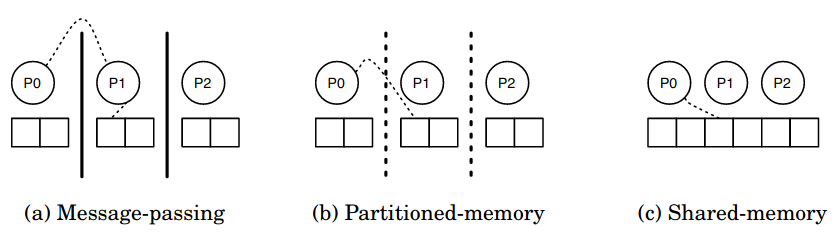
\includegraphics[width=\columnwidth]{mem_models.png}
    \caption{Modele pamięci~\cite{pgas_paper}}
    \label{fig:mem_models}
\end{figure}

Model PGAS cieszył się dużym wsparciem.
Powstało wiele rozszerzeń do języków, a nawet samodzielnych języków,
które umożliwiały z nim integrację.

\section{Języki modelu PGAS}

\subsection{CAF}
\label{ssec:caf}

Coarray Fortran (CAF)~\cite{coarray_fortran} jest rozszerzeniem Fortrana 95/2003,
który wprowadza elementy programowania równoległego.
Pozwala definiować tablice rozpięte na wszystkie \textit{obrazy}.
Obrazem nazywana jest kazda rozdystrybuowana kopia programu.
Ponadto pozwala na takie rzeczy jak synchronizacja wszystkich obrazów
lub dostęp do ich identyfikatorów.
Nie jest on wspierany od ponad 10 lat.

\subsection{Titanium}

\begin{figure}
    \centering
    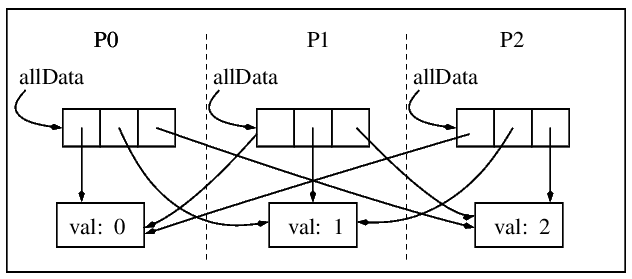
\includegraphics[width=\columnwidth]{titanium_memory.png}
    \caption{Przykładowy schemat pamięci dla tablicy rozpiętej na trzech procesach~\cite{titanium_docs}}
    \label{fig:titanium_memory}
\end{figure}

Titanium~\cite{titanium} jest dialektem Javy, który
pozwala na wprowadzenie abstrakcji nad równoległością.
Uniemożliwia on bezpośrednie używanie wątków, ale za to udostępnia
takie mechanizmy jak:
\begin{itemize}
    \item bariery,
    \item zmienne współdzielone między procesami,
    \item rozgłaszanie zmiennych pomiędzy procesy,
    \item tablice rozpięte na wszystkich procesach,
\end{itemize}
oraz wiele innych.
Ostatnia jego wersja była kompatybilna z Javą 1.4.
Przykładowy schemat tablicy w Titanium jest
przedstawiony na rysunku~\ref{fig:titanium_memory}.

\subsection{UPC}

Unified Parallel C (UPC)~\cite{upc} jest rozszerzeniem do języka C,
który wprowadza elementy programowania równoległego.
Podstawowe cechy:
\begin{itemize}
    \item Model wykonywania SPMD --- Single Program Multiple Data.
    \item Stała liczba tzw.\ \textit{places} nazywanych tutaj wątkami.
    Może być wybrana statycznie --- podczas kompilacji lub dynamicznie --- podczas wykonania.
    \item Domyślnie deklarowane zmienne zmienna są prywatne.
    Jeżeli jakaś dana ma być wspóldzielona oznacza się ją słowem kluczowym \textit{shared}.
    \item Dostęp do danych prywatnych i współdzielonych następuje w ten sam sposób.
    \item Posiada dodatkową instrukcję sterującą \texttt{upc\_forall}, za pomocą której
    możemy określić która iteracja pętli ma być wykonana przez który wątek.
\end{itemize}

Ostatnia wersja języka pochodzi z roku 2013~\cite{upc},
natomiast istnieje wiele implementacji, które są nadal
rozwijane~\cite{berkleyupc, upc_clang}.

\subsection{UPC++}

UPC++~\cite{upcxx} jest biblioteką do języka C++, która
pozwala na użycie modelu PGAS.
Podstawowe cechy:
\begin{itemize}
    \item aktywnie rozwijany --- ostatnia wersja wydana 12 marca 2020r.,
    \item jest odpowiednikiem UPC napisanym dla języka C++,
    \item ma dużo ciekawych funkcjonalności jak np.\ RPC (Remote Procedure Calls)
    czy początkowe wsparcie dla Nvidia CUDA~\cite{upcpp}.
\end{itemize}

\subsection{Chapel}

W przeciwieństwie do poprzednich narzędzi,
Chapel jest językiem programowania zaprojektowanym na potrzeby obliczeń równlogełych na wielką skalę.
Jego głównym założeniem implementacyjnym jest przenośność, która pozwala na uruchamianie go
na domowych komputerach i laptopach, klastrach oraz chmurach obliczeniowych oprócz wspieranych domyślnie
wydajnych superkomputerów, dla których został zaprojektowany.
Podstawowe cechy:
\begin{itemize}
    \item tzw. \textit{execution model} APGAS --- Asynchronous PGAS,
    \item zawiera mechanizmy \textit{implicit paralellism}, na przykład pętla \textit{forall},
    \item możliwe deklarowanie zmiennych w konkretnym \textit{place},
    \item wprowadza zarówno \textit{implicit} jak i \textit{explicit} \textit{remote data access},
    \item aktywnie rozwijany jako projekt open-source,
    \item posiada bogatą w przykłady dokumentację i materiały pozwalające na szybką
    i prostą naukę.
\end{itemize}

\subsection{XCalableMP}

Rozszerzenie dla języka C i Fortran przypominające OpenMP.
Wzorowane na HPF (High Performance Fortran~\cite{pgas_paper}) oraz
CAF (Co-array Fortran, opisany w sekcji~\ref{ssec:caf}).
Jest to zbiór dyrektyw kompilatora.
Podstawowe cechy:
\begin{itemize}
    \item Model wykonywania SPMD --- Single Program Multiple Data
    \item \textit{Explicit data distribution} oraz \textit{explicit remote data access}
    \item ostatnia specyfikacja pochodzi z listopada 2018 roku~\cite{xmphome}
\end{itemize}

\section{Wstępna analiza wybranych narzędzi}

\subsection{UPC++}

Instalacja biblioteki UPC++ nie jest trywialna.
Należy skompilować ją ze źródeł, gdyż nie jest ona udostępniania w postaci
binarnej na żadną dystrybucję.
Nie instaluje się ona również w standardowy sposób --- wykorzystuje ona własne
ścieżki w systemie (np. \texttt{/usr/local/upcxx}).
Przez to nie integruje się ona w łatwy sposób ze standardowymi narzędziami,
oraz wymaga ona własnego wrappera na kompilator (o nazwie \texttt{upcxx}).

Aby uruchomić skompilowany kod, należy użyć narzędzia \texttt{upcxx-run},
które jako jeden z argumentów przyjmuje liczbę procesów, na których uruchomić kod.
Jest to mały skrypt Pythonowy, pomagający w równoległym uruchomieniu programu.

Samo pisanie kodu za pomocą UPC++ jest analogiczne do używania
zwykłej biblioteki C++.
Kod korzystający z funkcji UPC++ musi być otoczony wywołaniami funkcji
\texttt{upcxx::init()} oraz \texttt{upcxx::finalize()}.
Większość funkcji dostępna jest z kontekstu statycznego z
przestrzeni nazw \texttt{upcxx}.
Przykładowe funkcje:
\begin{description}
\item[\texttt{upcxx::rank\_n()}] funkcja zwracająca liczbę wszystkich procesów,
\item[\texttt{upcxx::rank\_me()}] funkcja zwracająca identyfikator procesu,
\item[\texttt{upcxx::barrier()}] funkcja synchronizująca wszystkie procesy do tego miejsca
(analogiczna do standardowych funkcji OpenCL lub CUDA).
\end{description}

UPC++ również udostępnia parę typów, które ułatwiają zarządzanie pamięcią.
Na przykład \texttt{upcxx::global\_ptr} definiuje wskaźnik na obiekt, który
przechowywany jest w pamięci współdzielonej danego procesu.
Proces, który zdefiniował dany wskaźnik globalny może go
przekonwertować do wskaźnika standardowego C++ i używać
bez wykonywania specjalnych funkcji.
Jeśli natomiast dany proces nie jest właścicielem pamięci,
Jeśli stworzył on ten wskaźnik to jest go w stanie
musi użyć funkcji \texttt{upcxx::rget} i \texttt{upcxx::rput} aby
odpowiednio odczytać i zapisać wartość obiektu.

Aby rozdystrybuować wskaźnik na inne procesy, należy
użyć typu \texttt{upcxx::dist\_object}, który pozwala pobrać
wskaźnik z dowolnego innego procesu.
Służy do tego metoda \texttt{fetch}.
Przykład kodu dostępny jest na listingu~\ref{lst:upcxx-example}.

\begin{lstlisting}[
    caption=Korzystanie z pamięci współdzielonej w UPC++,
    label={lst:upcxx-example}]
upcxx::global_ptr<int> variable_ptr =
    upcxx::new_<int>(42);
upcxx::dist_object<upcxx::global_ptr<int>>
    variable(variable_ptr);

// variable from process 0
upcxx::global_ptr<int> variable_0 =
    variable.fetch(0).wait();
// variable from process 1
upcxx::global_ptr<int> variable_1 =
    variable.fetch(1).wait();
\end{lstlisting}

Obiekty typu \texttt{upcxx::future} są wszechobecne
i reprezentują klasyczne future'y.
Zwracane są one w przypadku uruchamiania funkcji
i metod, które mogą nie być natychmiastowe,
na przykład pobieranie wartości zmiennej z innego
procesu lub wykonanie RPC.

Przykład zastosowania tego drugiego obrazuje listing~\ref{lst:upcxx-rpc-example}.
\begin{lstlisting}[
    caption=Zastosowanie RPC w UPC++,
    label={lst:upcxx-rpc-example}]
upcxx::future<int> fut_result =
    upcxx::rpc(n, square, 2, 3);
int result = fut_result.wait();
\end{lstlisting}
Funkcja \texttt{square} jest funkcją wyliczającą pole prostokąta.
Do funkcji \texttt{upcxx::rpc()} przekazujemy nr procesu, na którym
ma zostać wykonana funkcja, nazwę samej funkcji, oraz jej argumenty.

W przypadku kiedy wykonujemy wiele obliczeń asynchronicznie,
zarządanie wszystkimi future'ami może być dosyć ciężkie, dlatego
UPC++ umożliwia grupowanie future'ów celem ich łatwiejszego zarządzania.
\begin{lstlisting}[
    caption=Grupowanie future w UPC++,
    label={lst:upcxx-conjoining-future}]
upcxx::future<int> fut_all =
    upcxx::make_future();
for (long i = 0; i < N; i++) {
    upcxx::future<int> fut =
        upcxx::rpc(n, square, 2, 3);
    fut_all =
        upcxx::when_all(fut_all, fut);
    if (i % 10 == 0) upcxx::progress();
}
fut_all.wait();
\end{lstlisting}
Listing~\ref{lst:upcxx-conjoining-future} przedstawia przykładowe wykorzystanie
wspomnianego mechanizmu. Najpierw zlecamy w pętli wykonanie pewnych obliczeń, łącząc
po każdym zleceniu nowo powstały futre z poprzednimi.
Na końcu wywołujemy \texttt{wait()}
na grupie future, powodując zablokowanie wykonania programu do czasu aż będzie
można odczytac wyniki z każdego future.

Przy wykorzystaniu komunikacji asynchronicznej pomocne są również tzw.\ \textit{callbacki}.
Listing \ref{lst:upcxx-callback-example} przedstawia przykładowe wykorzystanie
mechanizmu callbacków w UPC++.
\begin{lstlisting}[
    caption=Wykorzystanie callbacku w UPC++,
    label={lst:upcxx-callback-example}]
upcxx::future<> fut = map.find(key).then(
    // lambda to check the return value
    [key](string val) {
        assert(val == key);
    });
\end{lstlisting}

UPC++ udostępnie również tzw.\ \textit{atomics}.
Umożliwiąją one atomowe wykonywanie operacji na
współdzielonych obiektach.
\begin{lstlisting}[
    caption=Atomics w UPC++,
    label={lst:upcxx-atomics-example}]
upcxx::atomic_domain<int64_t> ad({
    upcxx::atomic_op::load,
    upcxx::atomic_op::add
});
ad.add(
    remote_array,
    local_array[i],
    memory_order_relaxed
).wait();
int64_t new_local_array = ad.load(
    *local_array,
    memory_order_relaxed
).wait();
\end{lstlisting}
Listing~\ref{lst:upcxx-atomics-example} przedstawia przykładowe użycie wspomnianego mechanizmu.
Najpierw inicjalizujemy nową \textit{atomic\_domain}.
Jest to wrapper na pewien typ, dostarczający pewnych operacji na tym typie.
Tutaj deklarujemy operacje \textit{load} oraz \textit{add}.
Do wspieranych typów należą \textit{float}, \textit{double} oraz \textit{signed/unsigned int32/64}.
Następnie wykonujemy operacje \texttt{add} i \texttt{load}, które w sposób atomowy odpowiednio
modyfikują tablicę znajdującą się w przestrzeni adresowej innego procesu oraz odczytują lokalną
tablicę upewniając się, że żaden inny proces jej właśnie nie modyfikuje.

UPC++ daje dużą swobodę i kontrolę programiście, co może być uznane
zarówno za zaletę jak i za wadę.
Zaletą jest większy wpływ na to co się dzieje.
Biblioteka nie tworzy sama z siebie żadnych
systemowych wątków, niewidocznych dla programisty, np.\ do obsługi
\textit{callbacków}.
Z jednej strony zyskujemy dzięki temu na wydajności
ale z drugiej jesteśmy zmuszeni ręcznie obsługiwać pewne mechanizmy
(w tym kontekście szczególnie ważne jest pojęcie \textit{progressu} oraz
umiejętne korzystanie z funkcji \texttt{upcxx::progress()}).
Podąrzając tym
tropem w UPC++ mamy tylko i wyłącznie tzw.\ \textit{explicit shared memory access}.
Twórcom biblioteki zależało na świadomym odwoływaniu się do danych, które należą do
innego procesu, co niesie ze sobą duży narzut wydajnościowy.
Niewątpliwą zaletą jest asynchroniczność biblioteki.
Większość udostępnianych
przez nią operacji wykonywanych jest właśnie w ten sposób.
Dostępność dobrej dokumentacji oraz ciągłe wsparcie również powinny
przyczynić się do skorzystania z UPC++.
Dużym minusem jest wymóg znajomości sposobu zarządzania pamięcią
w C++ aby efektywnie używać tej biblioteki.

\subsection{Chapel}

Instalacja kompilatora Chapel nie stanowi większego problemu.
Jest on dostępny w formie gotowych bibliotek na systemy Cray i
MacOS oraz jako obraz Dockera.
Możliwa jest też instalacja ze źródeł, która sprowadza się do uruchomienia polecenia
\texttt{make} oraz aktywacji zmiennych poleceniem \texttt{source}.

Po przygotowaniu narzędzia w prosty sposób możemy skompilować przykładowy program:
\texttt{chpl -o hello examples/hello.chpl}, a następnie uruchomić go: \texttt{./hello}.
Składnia Chapel przywodzi na myśl języki C/C++ oraz Python.
Z niewielkim wysiłkiem można
pisać proste programy po przeczytaniu zaledwie kilku linijek dokumentacji lub przykładowych
programów.

\begin{lstlisting}[
    caption=Przykładowy kod wypisujący liczby od 1 do 1000 w Chapel,
    label={lst:chapel-iter}]
config const n = 1000;

forall i in 1..n do
    writeln("Hello from iter #", i);
\end{lstlisting}

Chapel dostarcza wiele elementów upraszczających programowanie równoległe.
Najciekawsze z nich to pętle \texttt{forall}, operacje filtrowania,
automatyczne tworzenie zmiennych lokalnych dla każdego z wątków oraz mechanizm promocji,
który jest zbliżony do znanej z biblioteki numpy techniki
broadcastingu pozwalającej na zastosowanie operacji skalarnej dla całej macierzy.


Implementacja obliczeń wielowątkowych polega na tworzeniu tzw. zadań, które
mogą zostać zdefiniowane poprzez polecenie \texttt{begin}, które w sposób nieustrukturyzowany
tworzy nowe zadanie.
Dodatkowo, możemy wykorzystać kwalifikatory \texttt{sync} oraz \texttt{single}
do zapewnienia synchronizacji między wątkami.
Chapel dostarcza również konstrukcje \texttt{cobegin} i \texttt{coforall}, które pozwalają
na równoległe wykonanie w nieco bardziej ustrukturyzowany sposób.
Tworzą one grupy zadań, a następnie zatrzymują się dopóki wszystkie zadania nie zostaną
wykonane.

Oprócz nich możemy wykorzystać kwalifikatory \texttt{sync} i \texttt{serial},
które pozwalają na tymczasowe przejście w tryb sekwencyjny.
Synchronizacja między wątkami może zostać zrealizowana poprzez zmienne współdzielone,
które zmodyfikować można tylko, gdy znajdują się w określonym stanie.
W przeciwnym wypadku wątek dokonujący modyfikacji zostanie wstrzymany do czasu osiągnięcia
przez zmienną oczekiwanego stanu.
Wspierane jest również kilka typów zmiennych, które pozwalają na wykonywanie na nich operacji
w sposób atomiczny.
Aktualnie są to zmienne boolowskie i wszystkie rozmiary liczb całkowitych oraz rzeczywistych.

\subsection{Opis benchmarków}

Dla każdej osoby został wybrany jeden benchmark:
\begin{description}
\item[wyznacznik macierzy] obliczanie wyznacznika dużych macierzy na wielu
procesach,
\item[mnożenie macierzy] mnożenie dwóch dużych macierzy na wielu procesach,
\item[obliczanie `stencila'] benchmark zaproponowany w dokumentacji UPC++,
który polega na równoległym operowaniu na jednowymiarowej tablicy, ustalając jej
stan z czasem, na przykład obliczanie elementu jako średniej jego sąsiadów.

\end{description}


\printbibliography
\end{document}
